\newpage
\section{Soal 7: Optimasi Multi-output Energy Efficiency dengan PSO}

Dataset D3 Energy Efficiency berisi 768 bangunan hasil simulasi dengan 8 fitur dan dua target, Heating Load ($Y_1$) dan Cooling Load ($Y_2$). PSO dijalankan dengan \texttt{pyswarms}.

\subsection{Business Understanding}
Sebelum gedung dibangun, arsitek perlu perkiraan beban pemanas dan pendingin untuk menentukan ukuran AC atau heater dan biaya operasionalnya. Simulasi detail itu lambat, jadi yang dicari di sini adalah semacam kalkulator kasar: dua model linear yang koefisiennya dicari PSO sekaligus dalam satu partikel.

\begin{tabularx}{\textwidth}{@{}LL@{}}
\toprule
\textbf{Kriteria kesuksesan} & \textbf{Ambang} \\
\midrule
PSO mendekati solusi analitik OLS di data latih & $J_{PSO} \leq 1.01 \times J_{OLS}$ \\
$R^2$ test masing-masing target & $\geq 0.85$ \\
Error relatif & RMSE $\leq 0.4\,\sigma$ target \\
\bottomrule
\end{tabularx}

\subsection{Data Understanding dan Data Preparation}
Data simulasi ini rapi: tidak ada missing value, duplikat, ataupun outlier menurut aturan IQR. Heating dan Cooling berkorelasi sangat kuat (0.976), dan distribusi keduanya punya dua puncak karena \emph{Overall\_Height} hanya bernilai 3.5 m atau 7 m.

Masalah terbesarnya multikolinearitas. Relative\_Compactness dan Surface\_Area berkorelasi $-0.99$, sedangkan Roof\_Area dan Overall\_Height $-0.97$. Lebih dari itu, Surface\_Area persis sama dengan Wall\_Area + 2 $\times$ Roof\_Area, sehingga rank matriks fitur hanya 7, padahal fiturnya 8.

Data dibagi 60/20/20. Train dipakai PSO, validation untuk memilih strategi batas, dan test hanya sekali di akhir. Fitur dan target distandardisasi dengan mean dan std data latih. Orientation dan Glazing\_Area\_Distribution tetap diperlakukan sebagai angka karena soal meminta model linear 8 fitur.

\fig{soal_07_1.png}{1.0}{Distribusi target, hubungan $Y_1$ dengan $Y_2$, dan Heating Load per tinggi gedung.}

\jawab{Jawaban 7a: Normalisasi RMSE dengan $\sigma$ dan dimensi partikel}
\[ J = \frac{\mathrm{RMSE}_{Y_1}}{\sigma_{Y_1}} + \frac{\mathrm{RMSE}_{Y_2}}{\sigma_{Y_2}} \]
Sebaran kedua target berbeda ($\sigma_{Y_1} = 10.07$ dan $\sigma_{Y_2} = 9.44$ di data latih). Kalau RMSE langsung dijumlahkan, target dengan angka lebih besar akan menguasai objective dan PSO hanya sibuk memperbaiki target itu. Setelah dibagi $\sigma$, RMSE menjadi ukuran ``berapa kali simpangan baku'' tanpa satuan. Nilai 1.0 berarti sama buruknya dengan selalu menebak rata-rata. Mirip nilai ujian dari dua dosen dengan skala berbeda yang harus dikonversi ke skala yang sama dulu sebelum dijumlah. Ukuran ini juga terhubung langsung dengan $R^2$ lewat $\mathrm{RMSE}/\sigma = \sqrt{1 - R^2}$.

Setiap model linear punya 8 bobot dan 1 bias, jadi satu partikel berdimensi $2 \times (8 + 1) = 18$ dengan susunan $[w^{(1)}_{1..8}, b_1, w^{(2)}_{1..8}, b_2]$.

\jawab{Jawaban 7b: Desain PSO dan \emph{boundary handling}}
Di setiap iterasi, kecepatan partikel diperbarui dari inersia, ingatan pribadi, dan tarikan kawanan:
\[ v \leftarrow w\,v + c_1 r_1 (p_{best} - x) + c_2 r_2 (g_{best} - x), \qquad x \leftarrow x + v \]

\begin{tabularx}{\textwidth}{@{}llL@{}}
\toprule
\textbf{Parameter} & \textbf{Nilai} & \textbf{Alasan} \\
\midrule
Partikel / iterasi & 40 / 300 & sekitar 2$\times$ dimensi; kurva sudah datar jauh sebelum iterasi 300 \\
$w$ & 0.7 & nilai konstan yang umum, mendekati 0.729 dari analisis Clerc \& Kennedy \\
$c_1 = c_2$ & 1.5 & ingatan pribadi dan pengaruh kawanan seimbang \\
Batas posisi & $[-3, 3]$ & data terstandardisasi, koefisien wajar sekitar $\pm$1; mencegah koefisien liar \\
Velocity clamp & $[-1, 1]$ & maksimal 1/6 lebar ruang per langkah \\
\bottomrule
\end{tabularx}

Clipping (\texttt{nearest}) menempelkan partikel yang keluar ke dinding terdekat, misalnya 3.7 menjadi 3.0. Caranya sederhana dan cocok kalau optimum ada di dekat batas, tetapi partikel bisa menumpuk di dinding sehingga keragaman swarm berkurang. Reflection (\texttt{reflective}) memantulkan partikel sejauh kelebihannya, jadi 3.7 menjadi 2.3. Partikel tetap bergerak dan keragaman terjaga, hanya saja partikel sulit diam tepat di batas kalau optimum memang ada di sana.

Keduanya saya uji dengan 5 seed per strategi:

\begin{adjustbox}{max width=\textwidth}\begin{tabular}{@{}lcccc@{}}
\toprule
& \textbf{$J$ train akhir} & \textbf{$J$ validation} & \textbf{$J$ train iterasi 20} & \textbf{Menempel di dinding (iter.~10)} \\
\midrule
Clipping & $0.6336 \pm 0.0040$ & $0.6343 \pm 0.0030$ & 1.111 & 1.2\% (puncak 4.4\%) \\
Reflection & $0.6327 \pm 0.0036$ & $0.6348 \pm 0.0035$ & 1.203 & 0\% \\
\bottomrule
\end{tabular}\end{adjustbox}

\fig{soal_07_3.png}{1.0}{Kiri: konvergensi gbest untuk 5 seed per strategi. Kanan: porsi koordinat partikel yang menempel di batas $\pm$3.}

Clipping memang membuat sebagian partikel menempel di dinding, tetapi hanya di awal pencarian dan jumlahnya kecil. Hasil akhirnya praktis sama, dengan selisih $J$ validation 0.0005, jauh di bawah variasi antar-seed. Penyebabnya, optimum OLS (sekitar $\pm$0.8) berada jauh di dalam batas $\pm$3. Strategi dipilih dari $J$ validation terkecil, yaitu clipping.

\jawab{Jawaban 7c: RMSE, $R^2$, dan \emph{convergence curve}}
\begin{adjustbox}{max width=\textwidth}\begin{tabular}{@{}lcccc@{}}
\toprule
\textbf{Target (test)} & \textbf{RMSE} & \textbf{MAE} & \textbf{$R^2$} & \textbf{RMSE/$\sigma$} \\
\midrule
Heating Load ($Y_1$) & 2.69 kWh/m$^2$ & 1.96 & 0.934 & 0.267 \\
Cooling Load ($Y_2$) & 3.27 kWh/m$^2$ & 2.18 & 0.892 & 0.346 \\
OLS pembanding (Heating / Cooling) & 2.70 / 3.28 & 1.98 / 2.20 & 0.933 / 0.891 & - \\
\bottomrule
\end{tabular}\end{adjustbox}

\begin{figure}[H]\centering
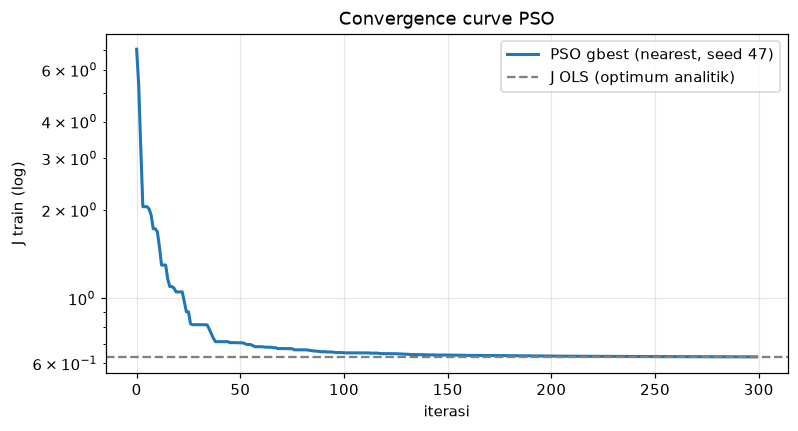
\includegraphics[width=0.42\textwidth]{figures/soal_07_4.png}\hfill
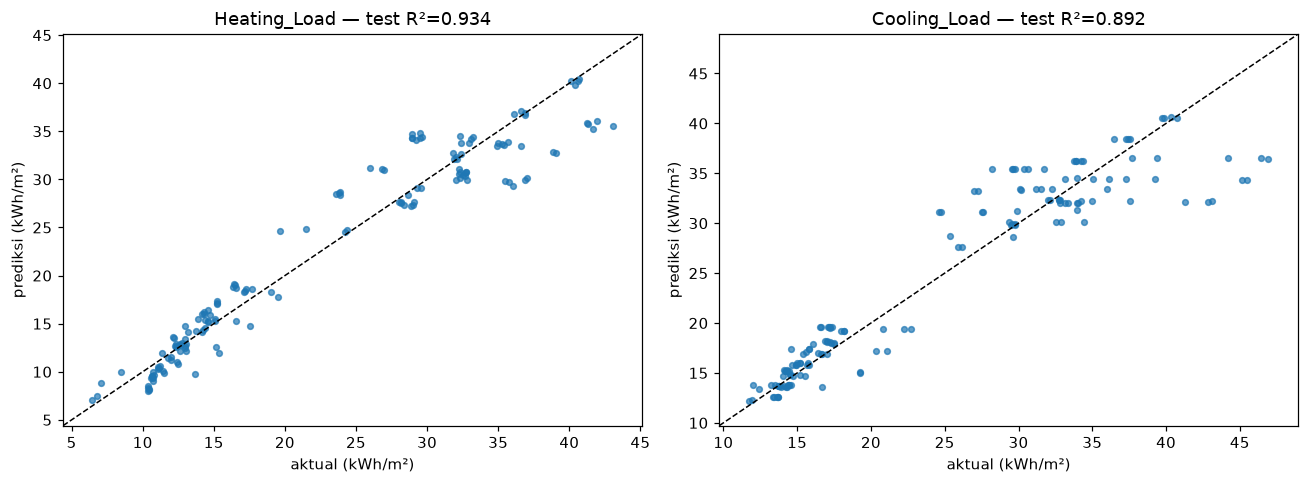
\includegraphics[width=0.56\textwidth]{figures/soal_07_5.png}
\caption{Kiri: \emph{convergence curve} PSO (seed 47) dibanding $J$ OLS. Kanan: prediksi vs aktual di test set.}
\end{figure}

$J$ test sebesar 0.613 hampir sama dengan train (0.632) dan validation (0.634), jadi model tidak overfit. PSO juga hampir mencapai optimum analitik: $J$ train 0.6321 dibanding 0.6302 milik OLS, hanya 0.3\% lebih buruk. Cooling lebih sulit diprediksi dan lebih menyebar di nilai tinggi, kemungkinan karena interaksi kaca dan tinggi gedung yang tidak bisa ditangkap model linear murni.

\jawab{Jawaban 7d: Fitur dominan dan keterbatasan interpretasi}
\begin{figure}[H]\centering
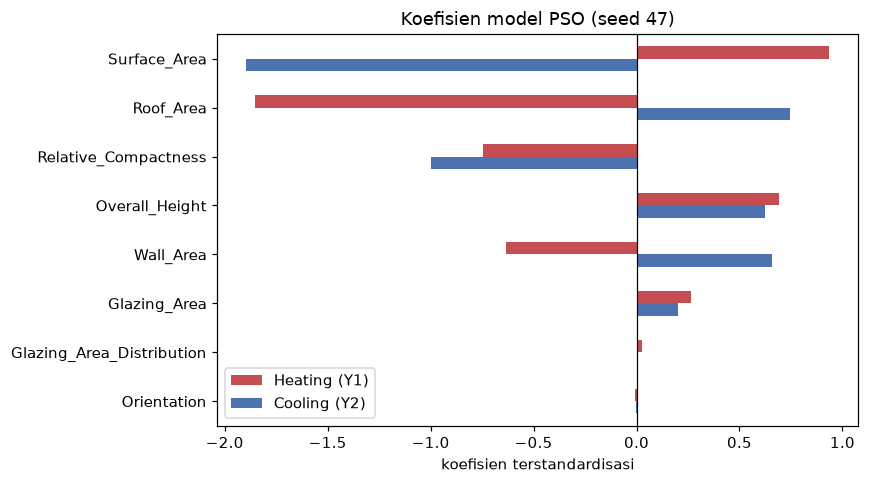
\includegraphics[width=0.55\textwidth]{figures/soal_07_6.png}
\caption{Koefisien terstandardisasi model PSO (seed 47).}
\end{figure}

\begin{adjustbox}{max width=\textwidth}\begin{tabular}{@{}lcccccc@{}}
\toprule
\textbf{Koef.\ Heating per seed} & \textbf{47} & \textbf{48} & \textbf{49} & \textbf{50} & \textbf{51} & \textbf{std} \\
\midrule
Relative\_Compactness & $-0.746$ & $-0.421$ & $-0.590$ & $0.096$ & $-0.462$ & 0.318 \\
Surface\_Area & 0.934 & $-0.445$ & 0.097 & 0.221 & $-0.933$ & 0.707 \\
Wall\_Area & $-0.632$ & 0.258 & $-0.120$ & 0.181 & 0.475 & 0.428 \\
Roof\_Area & $-1.853$ & 0.070 & $-0.733$ & 0.116 & 0.524 & 0.943 \\
Overall\_Height & 0.692 & 0.847 & 0.784 & 1.059 & 0.836 & 0.135 \\
Glazing\_Area & 0.264 & 0.265 & 0.269 & 0.275 & 0.268 & 0.004 \\
Orientation & $-0.009$ & $-0.008$ & $-0.007$ & $-0.006$ & $-0.006$ & 0.001 \\
\bottomrule
\end{tabular}\end{adjustbox}

Dua fitur bisa dipercaya sebagai fitur dominan. Overall\_Height selalu positif (0.69 sampai 1.06 di kelima seed), dan solusi OLS juga menempatkannya sebagai koefisien terbesar (+0.76 untuk Heating dan +0.80 untuk Cooling). Glazing\_Area sangat stabil dengan std antar-seed 0.004. Orientation tidak berpengaruh karena koefisiennya selalu mendekati nol.

Kalau koefisien seed 47 dibaca mentah, fitur paling dominan justru Surface\_Area dan Roof\_Area. Masalahnya, koefisien Roof\_Area bisa $-1.85$ di satu seed dan $+0.52$ di seed lain, padahal $J$ kelima seed hampir sama (0.630 sampai 0.640). Penyebabnya terlihat jelas saat koefisien (Surface, Wall, Roof) saya geser dari $(0.93, -0.63, -1.85)$ ke $(1.89, -1.12, -2.85)$: $J$ train tetap 0.632094 sampai 6 desimal. Karena Surface = Wall + 2 $\times$ Roof, ada tak terhingga kombinasi koefisien dengan prediksi yang identik. Seperti tiga orang yang mengangkat satu meja: berat totalnya selalu sama, tetapi pembagian beban per orang bisa berapa saja.

Magnitudo koefisien hanya sah dibandingkan kalau fitur-fiturnya tidak saling berkorelasi. Untuk dataset ini ada tiga jalan keluar: membuang fitur yang kolinear sempurna, menambah regularisasi L2 di objective agar solusinya unik, atau memakai \emph{permutation importance} per kelompok fitur.

\subsection{Interpretasi Hasil}
Pada 20 bangunan test, sebagian besar prediksi meleset 0 sampai 3 kWh/m$^2$. Kesalahan terbesar ada pada gedung tinggi dengan kaca 40\%, dengan Cooling aktual 46.4 dan prediksi 36.5. Ini kasus interaksi tinggi dan kaca yang tidak tertangkap model linear.

\begin{adjustbox}{max width=\textwidth}\begin{tabular}{@{}llll@{}}
\toprule
\textbf{Kriteria} & \textbf{Target} & \textbf{Hasil} & \textbf{Status} \\
\midrule
$J_{PSO} \leq 1.01\,J_{OLS}$ & $\leq 1.01$ & 1.0031 (4/5 seed; seed 50 = 1.016) & \ok{tercapai} \\
$R^2$ test Heating / Cooling & $\geq 0.85$ & 0.934 / 0.892 & \ok{tercapai} \\
RMSE $\leq 0.4\sigma$ & $\leq 0.4$ & 0.267 / 0.346 & \ok{tercapai} \\
\bottomrule
\end{tabular}\end{adjustbox}

Satu partikel 18 dimensi berhasil mengoptimasi dua model sekaligus dengan hasil yang praktis sama dengan OLS. Clipping dan reflection berakhir di model yang sama karena optimum jauh dari batas. Tinggi gedung dan luas kaca adalah fitur dominan yang bisa dipercaya, sedangkan koefisien fitur geometri lain tidak bisa ditafsirkan per fitur karena kolinear sempurna.
